% Overleaf-ready Capstone Thesis
% Replace every item marked [UPDATE] before final submission.
\documentclass[12pt,a4paper,oneside]{report}

\usepackage[margin=1in]{geometry}
\usepackage{times}
\usepackage[T1]{fontenc}
\usepackage[utf8]{inputenc}
\usepackage{graphicx}
\usepackage{amsmath,amssymb}
\usepackage{booktabs}
\usepackage{array}
\usepackage{longtable}
\usepackage{multirow}
\usepackage{float}
\usepackage{caption}
\usepackage{setspace}
\usepackage{enumitem}
\usepackage{url}
\usepackage[hidelinks]{hyperref}
\usepackage{fancyhdr}
\usepackage{titlesec}
\usepackage[numbers,sort&compress]{natbib}

\onehalfspacing
\setlength{\emergencystretch}{2em}
\setlength{\parindent}{0.5in}
\setlength{\parskip}{0pt}
\graphicspath{{figures/}}
\captionsetup{font=small,labelfont=bf}
\titleformat{\chapter}[display]{\bfseries\centering\Large}{CHAPTER \thechapter}{0.5em}{\Large}
\titleformat{\section}{\bfseries\large}{\thesection}{0.75em}{}
\titleformat{\subsection}{\bfseries\normalsize}{\thesubsection}{0.75em}{}
\pagestyle{fancy}
\fancyhf{}
\fancyfoot[C]{\thepage}
\renewcommand{\headrulewidth}{0pt}

\newcommand{\projecttitle}{Layer Contrastive Decoding and Epistemic Reliability Estimation for Hallucination Aware Small Language Models}
\newcommand{\guide}{Dr. Palacharla Ravi Kumar}
\newcommand{\department}{Computer Science and Engineering}
\newcommand{\studentone}{E. Ganesh Kumar Reddy}
\newcommand{\studenttwo}{B. Sai Susmitha}
\newcommand{\studentthree}{P. Dhanush Datta}
\newcommand{\studentfour}{E. Sri Vardhan Reddy}

\begin{document}
\pagenumbering{roman}

% ---------- Title page ----------
\begin{titlepage}
\begin{center}
{\Large\bfseries \projecttitle\par}
\vspace{0.75in}
{\large A CAPSTONE PROJECT REPORT\par}
\vspace{0.35in}
{\normalsize Submitted in partial fulfillment of the requirements for the award of the degree of\par}
\vspace{0.25in}
{\large\bfseries BACHELOR OF TECHNOLOGY\par}
{\large\bfseries IN COMPUTER SCIENCE AND ENGINEERING\par}
\vspace{0.45in}
{\normalsize by\par}
\vspace{0.15in}
\begin{tabular}{ll}
\studentone & [UPDATE REGISTRATION NUMBER]\\
\studenttwo & [UPDATE REGISTRATION NUMBER]\\
\studentthree & [UPDATE REGISTRATION NUMBER]\\
\studentfour & [UPDATE REGISTRATION NUMBER]\\
\end{tabular}
\vfill
{\normalsize Under the guidance of\par}
\vspace{0.12in}
{\large\bfseries \guide\par}
{\normalsize Assistant Professor Sr. Grade 2\par}
\vspace{0.65in}
{\large\bfseries SCHOOL OF COMPUTER SCIENCE AND ENGINEERING\par}
{\large\bfseries VIT-AP UNIVERSITY\par}
{\normalsize Amaravati - 522237, Andhra Pradesh\par}
\vspace{0.35in}
{\bfseries NOVEMBER 2026\par}
\end{center}
\end{titlepage}

% ---------- Certificate ----------
\chapter*{CERTIFICATE}
\addcontentsline{toc}{chapter}{Certificate}
\thispagestyle{plain}
\noindent This is to certify that the Capstone Project work titled \emph{\projecttitle} is being submitted by \studentone, \studenttwo, \studentthree, and \studentfour\ in partial fulfillment of the requirements for the award of the degree of Bachelor of Technology in \department. This report is a record of bona fide work carried out under my guidance. To the best of my knowledge, the contents of this report have not been submitted, in full or in part, to any other institute or university for the award of any degree or diploma.

\vspace{1.4in}
\noindent\begin{minipage}[t]{0.45\textwidth}
\textbf{\guide}\\
Project Guide
\end{minipage}\hfill
\begin{minipage}[t]{0.40\textwidth}
\textbf{[UPDATE HOD NAME]}\\
Head of Department\\
\department
\end{minipage}

\vfill
\noindent The thesis is satisfactory / unsatisfactory.\\[0.7in]
\noindent\begin{minipage}[t]{0.42\textwidth}\textbf{Examiner 1}\\[0.35in]Signature\end{minipage}\hfill
\begin{minipage}[t]{0.42\textwidth}\textbf{Examiner 2}\\[0.35in]Signature\end{minipage}
\clearpage

% ---------- Acknowledgement ----------
\chapter*{ACKNOWLEDGEMENT}
\addcontentsline{toc}{chapter}{Acknowledgement}
We express our sincere gratitude to VIT-AP University for providing the academic environment and infrastructure required to complete this Capstone Project. We thank the faculty and staff of the School of Computer Science and Engineering for their encouragement and support.

We are especially grateful to \guide, our project guide, for constructive guidance, technical feedback, and continued encouragement throughout the design, implementation, and evaluation of this work. We also thank our family members and friends for their patience and support.

\vspace{0.35in}
\noindent\textbf{Project Team Members}\par
\noindent \studentone -- [UPDATE REGISTRATION NUMBER]\par
\noindent \studenttwo -- [UPDATE REGISTRATION NUMBER]\par
\noindent \studentthree -- [UPDATE REGISTRATION NUMBER]\par
\noindent \studentfour -- [UPDATE REGISTRATION NUMBER]
\clearpage

% ---------- Abstract ----------
\chapter*{ABSTRACT}
\addcontentsline{toc}{chapter}{Abstract}
Small language models can generate fluent but unsupported answers. Token likelihood alone is not a calibrated measure of answer-level reliability. This project develops and audits a TinyLlama-1.1B pipeline that combines Decoding by Contrasting Layers (DoLa), an Epistemic Neural Network (ENN), and sampled self-consistency to support hallucination-aware response generation. The active implementation contrasts mature and dynamically selected premature hidden states, trains a frozen-prior epinet for next-token prediction on document-disjoint C4 features, and optionally aggregates multiple sampled answers.

The archived held-out evaluation contains 211 examples: 169 TruthfulQA and 42 HaluEval-QA examples, with 54 positive and 157 negative labels. A 2048-dimensional ENN representation achieved AUROC 0.691, AUPRC 0.513, and accuracy 0.782. At a conservative calibrated operating point, DoLa+ENN achieved accuracy 0.768, precision 0.647, recall 0.204, F1 0.310, expected calibration error 0.123, and a false-accept rate of 0.038. Self-consistency did not change those thresholded decisions. The study therefore supports uncertainty-aware abstention for applications that prioritize avoiding unreliable answers; it does not establish universal hallucination prevention. Missing upgraded training source files and class-imbalance-sensitive thresholding are documented as reproducibility and generalization limitations.

\noindent\textbf{Keywords:} small language models, hallucination detection, factuality, DoLa, epistemic neural networks, uncertainty estimation, self-consistency, calibration.
\clearpage

\tableofcontents
\listoffigures
\listoftables
\clearpage
\pagenumbering{arabic}

\chapter{INTRODUCTION}
\section{Background}
Large language models are used for question answering, summarization, and interactive assistance. Their training objective rewards likely continuations rather than truth, so a response may sound coherent while conflicting with evidence or repeating a misconception. TruthfulQA was designed to evaluate questions that entice language models to imitate common falsehoods \citep{lin2022truthfulqa}; HaluEval provides human-annotated hallucinated and normal samples \citep{li2023halueval}. This project investigates reliability mechanisms for a small, locally runnable language model.

Hallucination detection and hallucination mitigation are related but different. Detection assigns a reliability score or a decision to a generated answer. Mitigation changes token decoding, answer selection, or the response policy to reduce unreliable output. The proposed system keeps this distinction explicit: DoLa changes decoding, the ENN estimates uncertainty-related signals, and self-consistency aggregates sampled candidate answers.

\section{Problem Statement}
Small language models have practical advantages in local deployment but may be more vulnerable to factual errors. A system that simply returns the highest-likelihood answer cannot distinguish an informative response from a plausible unsupported one. The problem addressed in this project is to design and evaluate an inspectable pipeline that can generate answers, expose uncertainty signals, rank candidate outputs, and make conservative accept or abstain decisions.

\section{Objectives}
\begin{enumerate}[label=\arabic*.]
\item Implement layer-contrastive decoding for TinyLlama using mature and premature transformer representations.
\item Train an epinet with a frozen prior to produce epistemic uncertainty diagnostics for next-token prediction.
\item Add sampled self-consistency to compare and aggregate multiple candidate answers.
\item Evaluate reliability, calibration, false-accept risk, and component-level ablations on held-out question-answer examples.
\item Present the result through an interactive console that exposes the generation parameters, candidate outputs, and verification diagnostics.
\end{enumerate}

\section{Organization of the Report}
Chapter 2 reviews relevant work on hallucination, factuality, uncertainty, and self-consistency. Chapter 3 describes the proposed system and mathematical formulation. Chapter 4 presents implementation details and the user interface. Chapter 5 explains the experimental methodology. Chapter 6 discusses results. Chapter 7 concludes the report and outlines future work.

\chapter{LITERATURE SURVEY}
\section{Hallucination and Factuality}
Hallucination has been defined as conflict with external facts, lack of support from provided sources, or inconsistency with task context. Surveys note that evaluation results depend on the task definition, annotation protocol, and external evidence available to the evaluator \citep{ji2023survey,huang2024audit}. TruthfulQA measures answers to misconception-inducing questions, while HaluEval supports hallucination-recognition tasks using annotated examples \citep{lin2022truthfulqa,li2023halueval}.

\section{Decoding by Contrasting Layers}
DoLa uses contrast between mature and premature layer distributions to improve factuality without fine-tuning the base language model \citep{chuang2024dola}. Instead of treating each transformer layer as equally useful, it emphasizes knowledge that emerges in deeper layers. The implementation in this project dynamically selects a premature layer by Jensen-Shannon divergence and contrasts its logits with the mature-layer logits.

\section{Epistemic Neural Networks and Calibration}
Epistemic Neural Networks represent uncertainty by adding an epistemic index to a predictive model \citep{osband2021enn}. The active epinet in this project uses a frozen random prior plus a trainable indexed residual. Its native prediction target is the next token, so its entropy diagnostics must not be interpreted automatically as answer-correctness probabilities. Calibration assesses whether a confidence level matches observed correctness and should therefore be measured independently \citep{guo2017calibration}.

\section{Self Consistency}
Self-consistency samples multiple reasoning paths or outputs and selects the most consistent answer \citep{wang2023selfconsistency}. It can improve stability when several valid paths agree, but it can also produce a consensus around the same error. For this reason, the project reports self-consistency as a separate component and measures its contribution through ablation.

\chapter{PROPOSED SYSTEM}
\section{System Overview}
The system uses TinyLlama-1.1B-Chat-v1.0 as the frozen base model \citep{zhang2024tinyllama}. The architecture separates the executable active path from an archived answer-correctness benchmark. C4-derived token features are used to train the active epinet. At inference time, the question-answering path supports Base and DoLa generation, ENN uncertainty scoring, optional self-consistency, and a reliability decision.

\begin{figure}[H]
\centering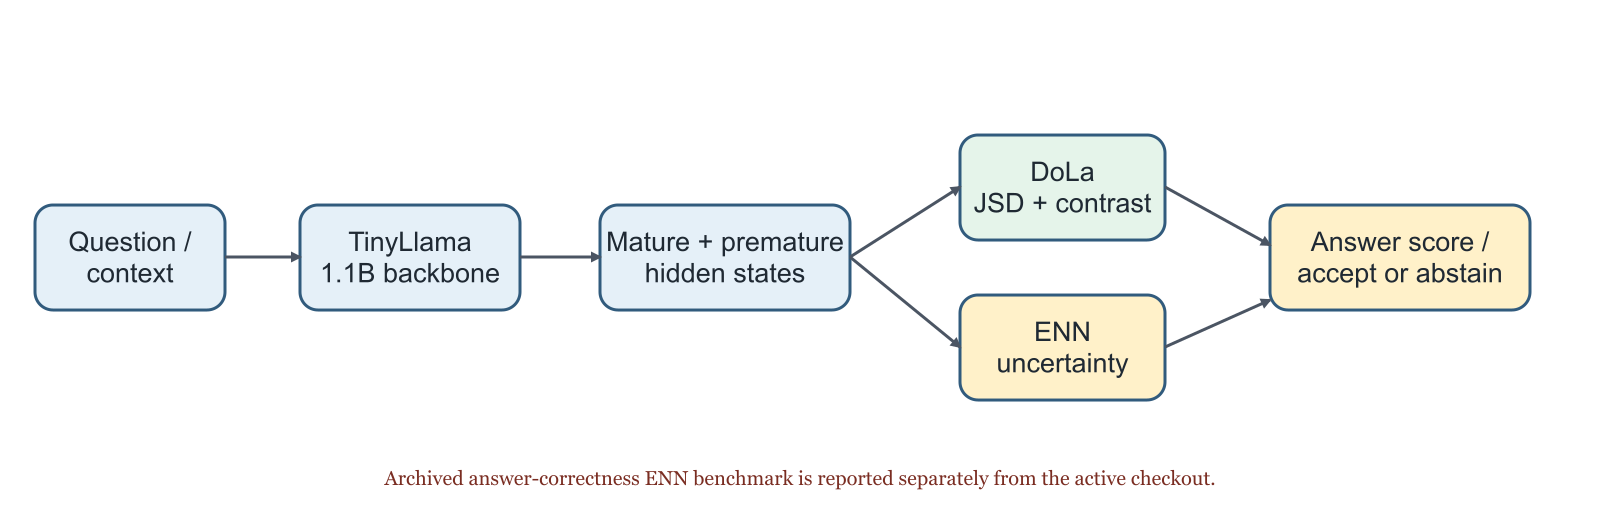
\includegraphics[width=0.92\textwidth]{architecture.png}
\caption{Active repository pipeline and the boundary to the archived answer-correctness benchmark.}
\label{fig:architecture}
\end{figure}

\section{DoLa Formulation}
For a token position $t$, let $h_t^m$ be the mature hidden state and $h_t^p$ be the selected premature hidden state. With language-model head matrix $W$ and contrast coefficient $\alpha$, the DoLa logits and distribution are
\begin{equation}
\ell_t^D = W h_t^m - \alpha W h_t^p, \qquad p_t^D = \operatorname{softmax}(\ell_t^D).
\end{equation}
The implementation considers candidate layers $\{0,4,8,12,16,20\}$ and uses block 21 as the mature layer. It selects the premature layer with the maximum Jensen-Shannon divergence from the mature distribution:
\begin{equation}
j_t^* = \arg\max_j \operatorname{JSD}\left(p_t^m\Vert p_t^j\right).
\end{equation}
The active default is $\alpha=0.05$. It is a configuration choice rather than a claimed optimum.

\begin{figure}[H]
\centering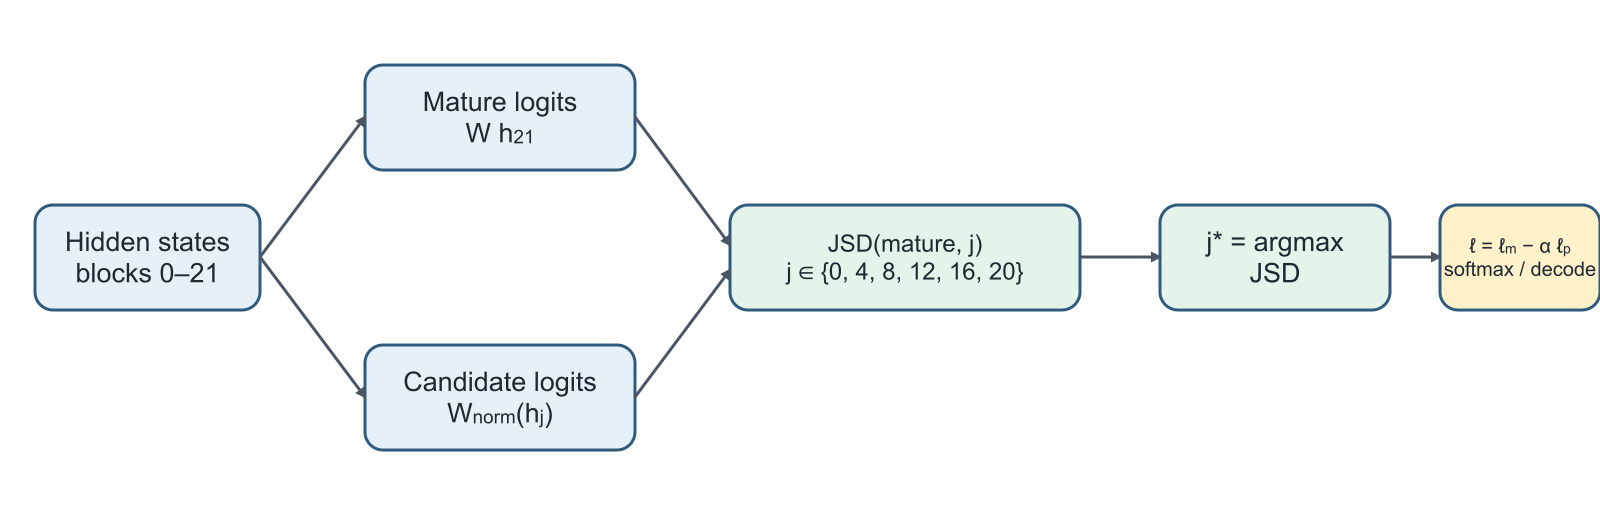
\includegraphics[width=0.86\textwidth]{dola_workflow.png}
\caption{DoLa workflow implemented in the active decoder.}
\label{fig:dola}
\end{figure}

\section{Epinet Architecture}
The epinet input concatenates mature and premature representations, $x_t=[h_t^m;h_t^p]\in\mathbb{R}^{4096}$. It uses a sampled epistemic index $z\sim\mathcal{N}(0,I_6)$, a frozen prior branch $f_0$, and a trainable branch $f_\phi$. The training objective is sampled next-token cross-entropy:
\begin{equation}
\mathcal{L}(\phi)=\frac{1}{|\mathcal{D}|K}\sum_{(x_t,y_t)\in\mathcal{D}}\sum_{k=1}^{K}
\operatorname{CE}\left(\ell_t^D+W[f_0(x_t,z_k)+f_\phi(x_t,z_k)],y_t\right).
\end{equation}
At inference, sampled distributions yield predictive entropy, expected entropy, and a nonnegative epistemic proxy. These values describe token distributions; a supervised, held-out evaluation is required before using them as answer-level confidence.

\begin{figure}[H]
\centering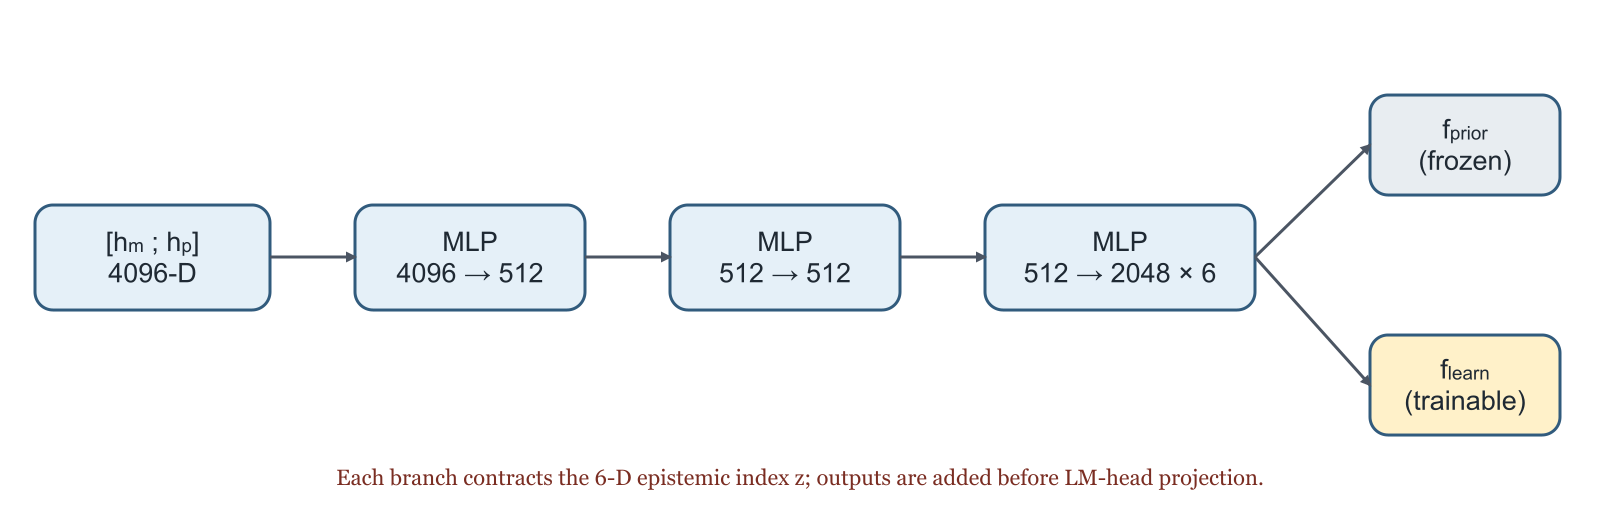
\includegraphics[width=0.86\textwidth]{epinet.png}
\caption{Active C4-trained epinet with a frozen prior and trainable indexed residual.}
\label{fig:epinet}
\end{figure}

\section{Candidate Aggregation and Reliability Decision}
For each prompt, the system can sample several DoLa candidates. Plain self-consistency normalizes answers and selects a plurality winner. An ENN-weighted version assigns an entropy-derived weight to each candidate. A separate reliability head or threshold policy can then accept the answer or return a conservative fallback. This design prevents token uncertainty, vote share, and answer correctness from being conflated.

\begin{figure}[H]
\centering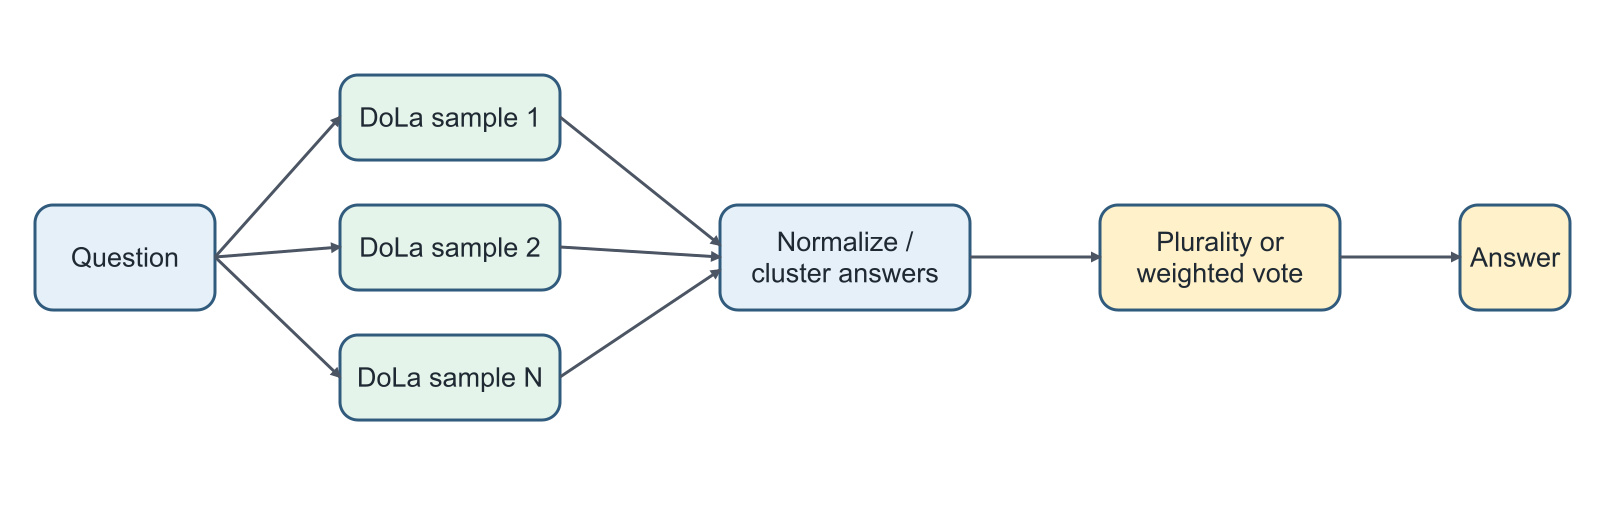
\includegraphics[width=0.86\textwidth]{self_consistency.png}
\caption{Candidate generation and self-consistency aggregation.}
\label{fig:selfconsistency}
\end{figure}

\begin{figure}[H]
\centering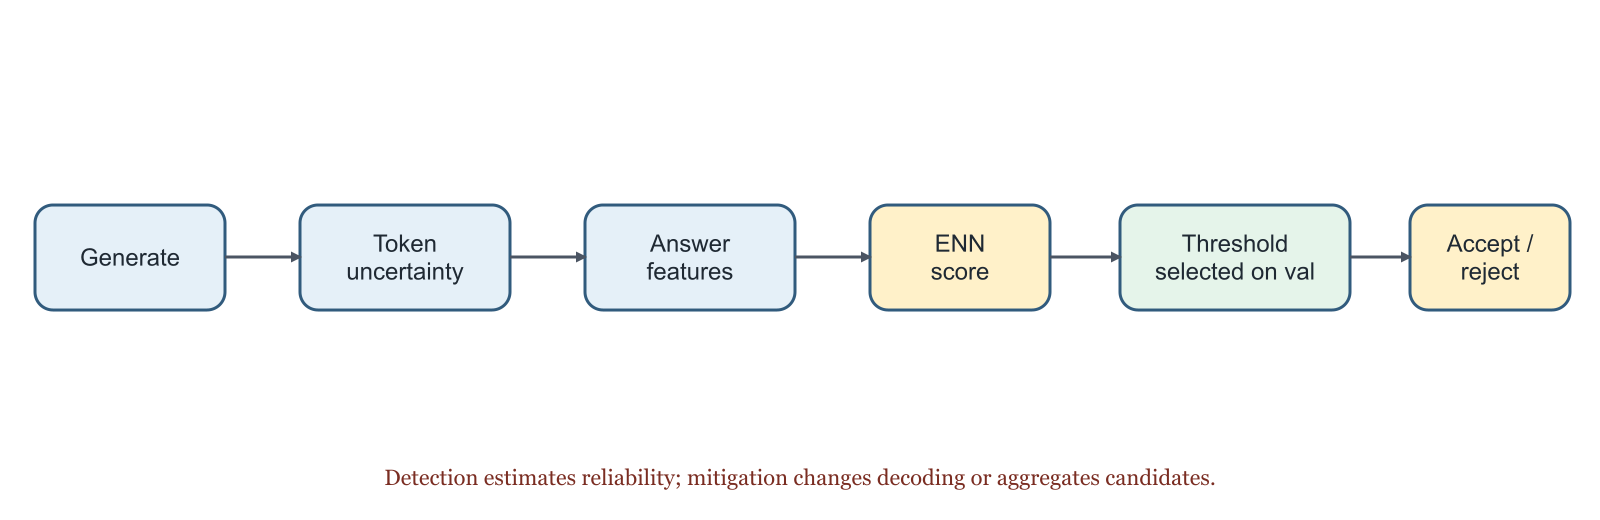
\includegraphics[width=0.86\textwidth]{detection_pipeline.png}
\caption{Detection scores and decides; mitigation changes decoding or answer aggregation.}
\label{fig:detection}
\end{figure}

\chapter{IMPLEMENTATION AND WORKING}
\section{Technology Stack}
The implementation uses Python, PyTorch, Hugging Face Transformers, the Datasets library, and a local TinyLlama checkpoint. The active project records Python 3.10.20, PyTorch 2.11.0, Transformers 5.17.0, Datasets 4.8.5, and Apple Silicon MPS in its environment audit. The interactive interface is implemented as a local web console.

\section{Training and Inference Flow}
The training path loads English C4 text, tokenizes sequences, extracts mature and dynamically selected premature hidden states, and creates next-token examples. A document-disjoint split prevents token positions from the same source document appearing in both training and validation sets. The saved full-cache run records 600 documents, 56,515 examples, a 90/10 split, batch size 32, learning rate $10^{-4}$, ten epochs, eight epistemic samples, and AdamW optimization.

During inference, a user question is encoded with the TinyLlama chat template. The application generates a base or DoLa answer, optionally samples additional candidates, computes diagnostic signals, aggregates candidates, and applies the configured verification policy. The output includes the selected answer and diagnostic information rather than an unqualified claim of factual correctness.

\section{Interactive Console}
Figure \ref{fig:console} shows the main console. The sidebar configures the generation length, temperature, nucleus sampling, DoLa contrast coefficient, self-consistency candidate count, and ENN weight. The main panel displays model status, a user prompt, the selected answer, a verification outcome, and component-level tabs for pipeline diagnostics, candidate agreement, claim analysis, token uncertainty, and retrieval evidence.

\begin{figure}[H]
\centering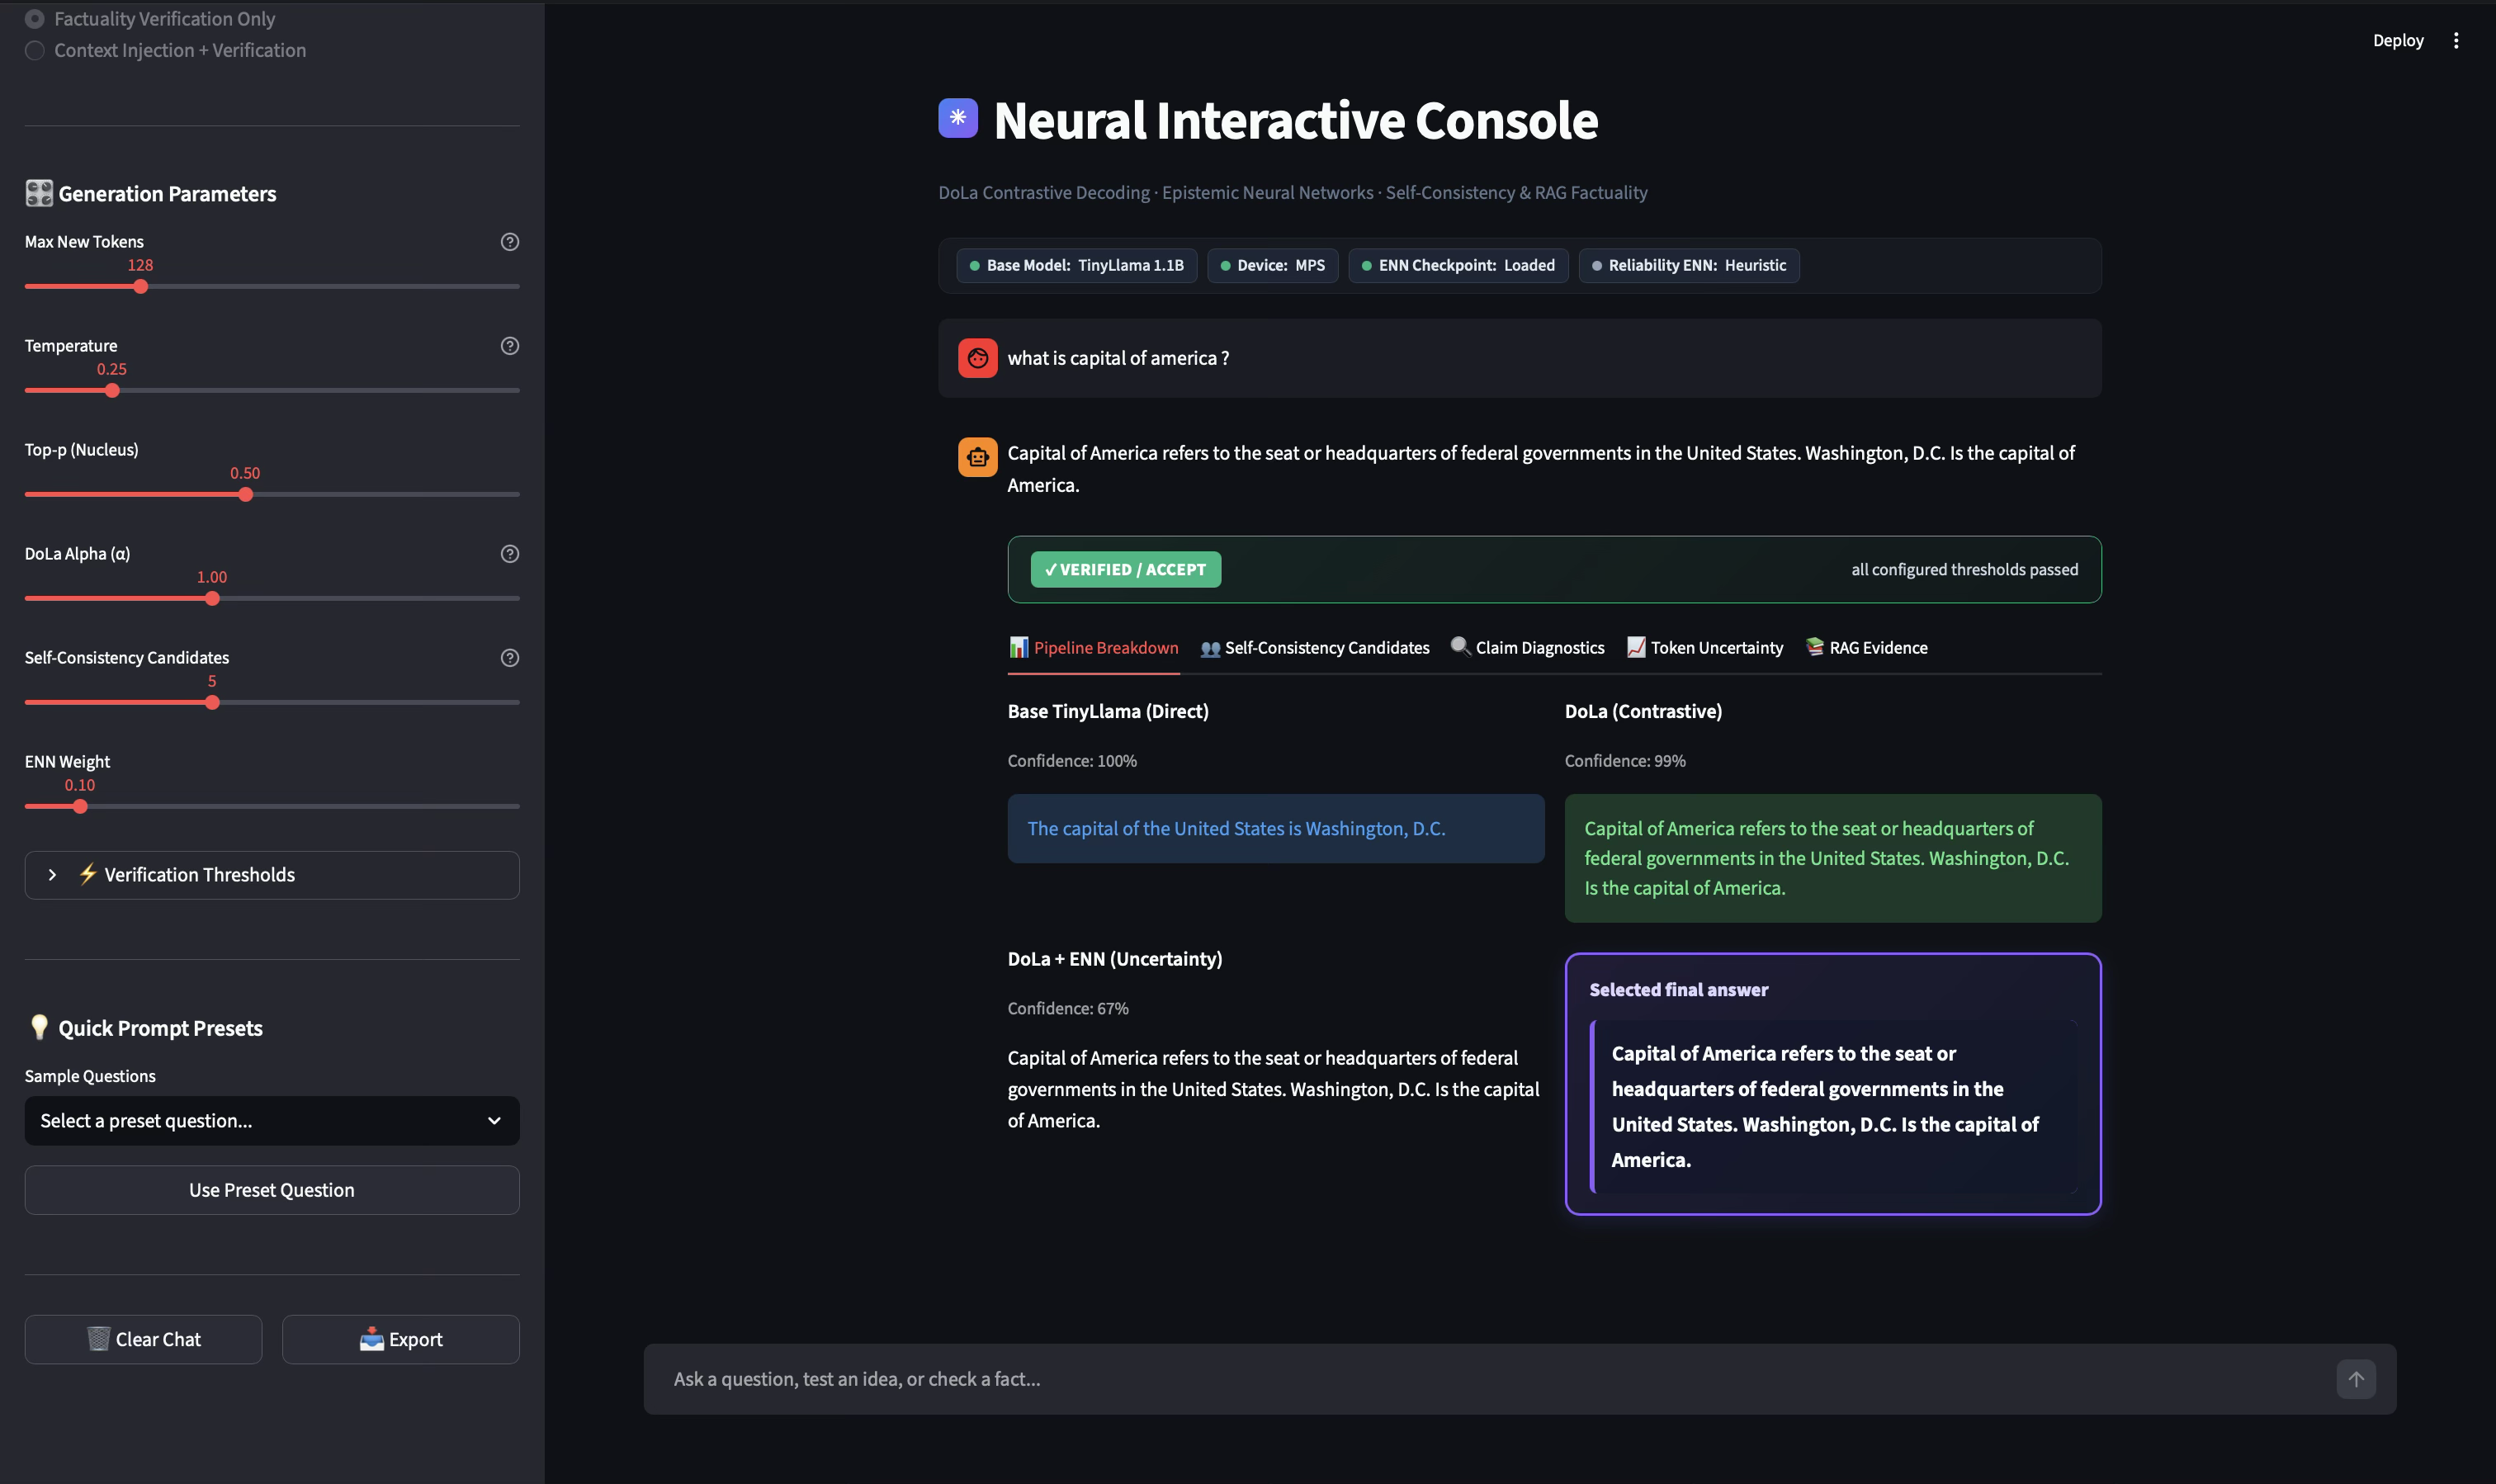
\includegraphics[width=\textwidth]{interactive_console.png}
\caption{Neural Interactive Console showing generation controls, selected answer, and verification diagnostics.}
\label{fig:console}
\end{figure}

Figure \ref{fig:candidates} shows the candidate-results view. It ranks sampled answers by final score and reports confidence, consensus, factuality, reliability, hallucination risk, verifier status, and an answer preview. This view enables an operator to inspect why an answer was accepted, rejected, or marked as a fallback.

\begin{figure}[H]
\centering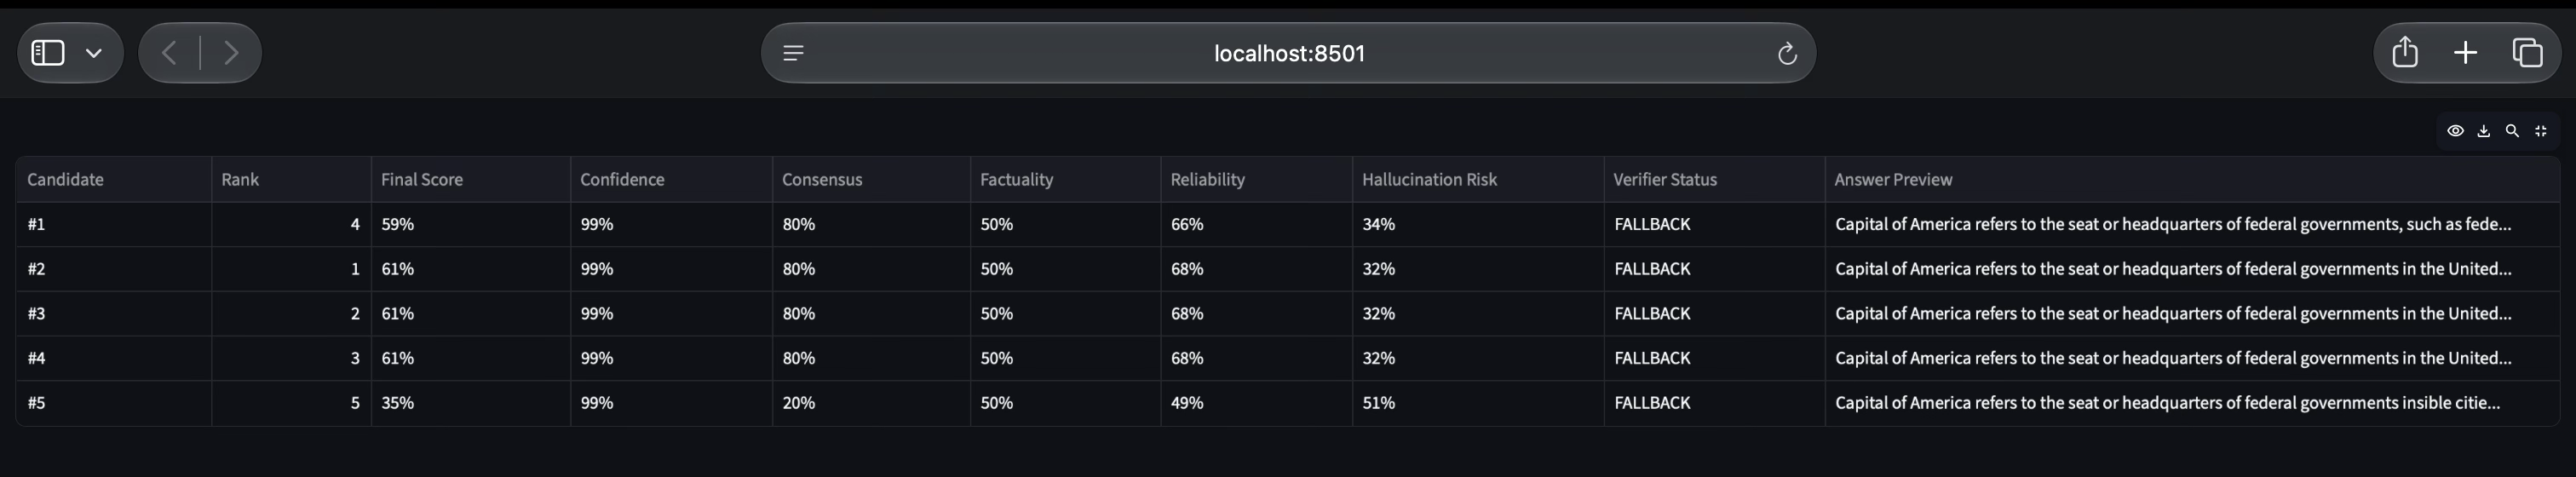
\includegraphics[width=\textwidth]{candidate_results.png}
\caption{Candidate-results interface with reliability and hallucination-risk diagnostics.}
\label{fig:candidates}
\end{figure}

\chapter{EXPERIMENTAL METHODOLOGY}
\section{Datasets and Protocol}
The archived held-out benchmark comprises 211 examples: 169 TruthfulQA and 42 HaluEval-QA examples. There are 54 positive examples defined by the project as reliable or correct and 157 negative examples. The report distinguishes active-source facts from archived results because the trainer source for the answer-correctness upgrade is not present in the current project checkout.

\section{Evaluation Metrics}
For a binary reliability decision, the study reports accuracy, balanced accuracy, precision, recall, F1, AUROC, AUPRC, expected calibration error (ECE), false-accept rate (FAR), and false-reject rate (FRR). FAR is particularly important for a conservative assistant because it measures the fraction of unreliable answers that are accepted. A low FAR can be achieved by rejecting many answers, so recall and FRR must be reported alongside it.

\begin{table}[H]
\centering
\caption{Verified active environment and archived benchmark inventory.}
\label{tab:inventory}
\begin{tabular}{p{0.28\textwidth}p{0.60\textwidth}}
\toprule
Item & Verified value or caveat\\ \midrule
Base model & TinyLlama-1.1B-Chat-v1.0; 22 layers, hidden size 2048, vocabulary size 32,000\\
Active ENN data & C4 cache: 600 documents and 56,515 token examples; document-disjoint 90/10 split\\
Archived held-out set & 211 examples: 169 TruthfulQA and 42 HaluEval-QA; 54 positive and 157 negative labels\\
Active training & Batch size 32; 10 epochs; learning rate $10^{-4}$; eight training index samples\\
Reproducibility caveat & Source for the archived upgraded answer-correctness trainer is absent from the active checkout\\
\bottomrule
\end{tabular}
\end{table}

\chapter{RESULTS AND DISCUSSION}
\section{Quantitative Comparison}
Table \ref{tab:results} summarizes the archived held-out comparison. Base TinyLlama and DoLa have high false-accept rates under the selected policy. Adding self-consistency improves accuracy and ECE relative to DoLa, but it accepts comparatively few positive examples. The conservative DoLa+ENN operating point substantially reduces FAR to 3.8\%, while its recall falls to 20.4\%. This is valuable for abstention-sensitive use cases but should not be described as universal correctness improvement.

\begin{table}[H]
\centering\scriptsize
\caption{Archived held-out comparison on 211 examples. Positive denotes the project-defined reliable or correct class.}
\label{tab:results}
\begin{tabular}{p{0.30\textwidth}rrrrrr}
\toprule
Method & Acc. & Prec. & Rec. & F1 & ECE & FAR\\ \midrule
Base TinyLlama & 28.4\% & 25.6\% & 94.4\% & 40.3\% & 45.8\% & 94.3\%\\
TinyLlama + DoLa & 29.9\% & 25.0\% & 87.0\% & 38.8\% & 39.5\% & 89.8\%\\
DoLa + self-consistency & 65.4\% & 34.4\% & 38.9\% & 36.5\% & 20.7\% & 25.5\%\\
DoLa + ENN-V2 & 76.8\% & 64.7\% & 20.4\% & 31.0\% & 12.3\% & 3.8\%\\
DoLa + ENN-V2 + SC & 76.8\% & 64.7\% & 20.4\% & 31.0\% & 12.3\% & 3.8\%\\
2048-D ENN alone & 78.2\% & 72.2\% & 24.1\% & 36.1\% & 11.6\% & 3.2\%\\
Complete combined & 72.5\% & 46.0\% & 42.6\% & 44.2\% & 19.5\% & 17.2\%\\
\bottomrule
\end{tabular}
\end{table}

\begin{figure}[H]
\centering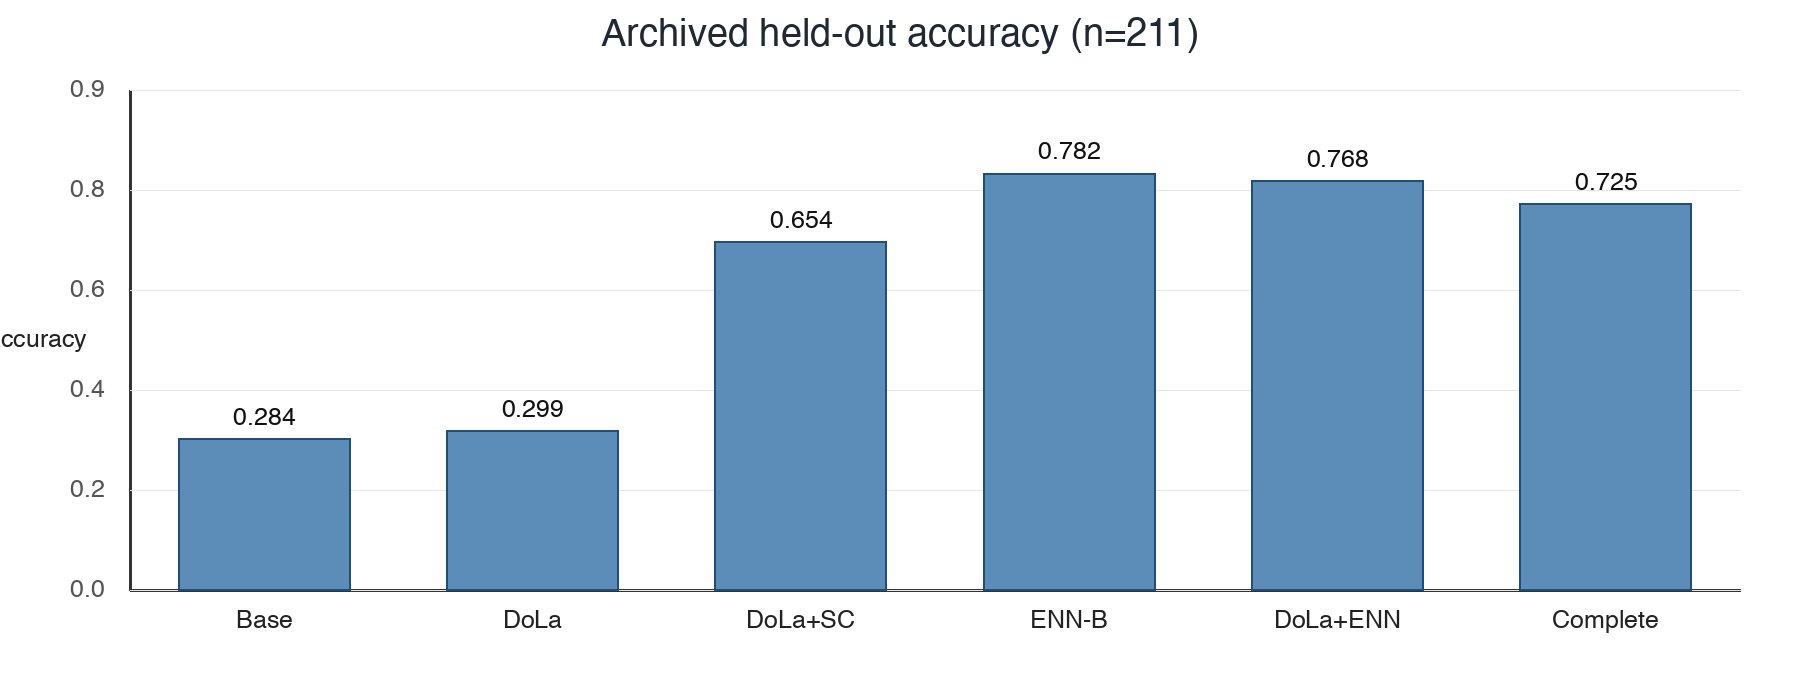
\includegraphics[width=0.80\textwidth]{performance.png}
\caption{Archived accuracy comparison across the evaluated architectures.}
\label{fig:performance}
\end{figure}

\section{Ablation Study}
The representation-only 2048-dimensional ENN produced AUROC 0.6681, while eight token diagnostics alone produced 0.3664 and six self-consistency features alone produced 0.5758. Combining representations, token diagnostics, and all self-consistency features produced AUROC 0.6713. The representation contains most of the discriminative signal; adding all components did not monotonically improve results. The saved DoLa+ENN and DoLa+ENN+self-consistency thresholded decisions are identical.

\begin{figure}[H]
\centering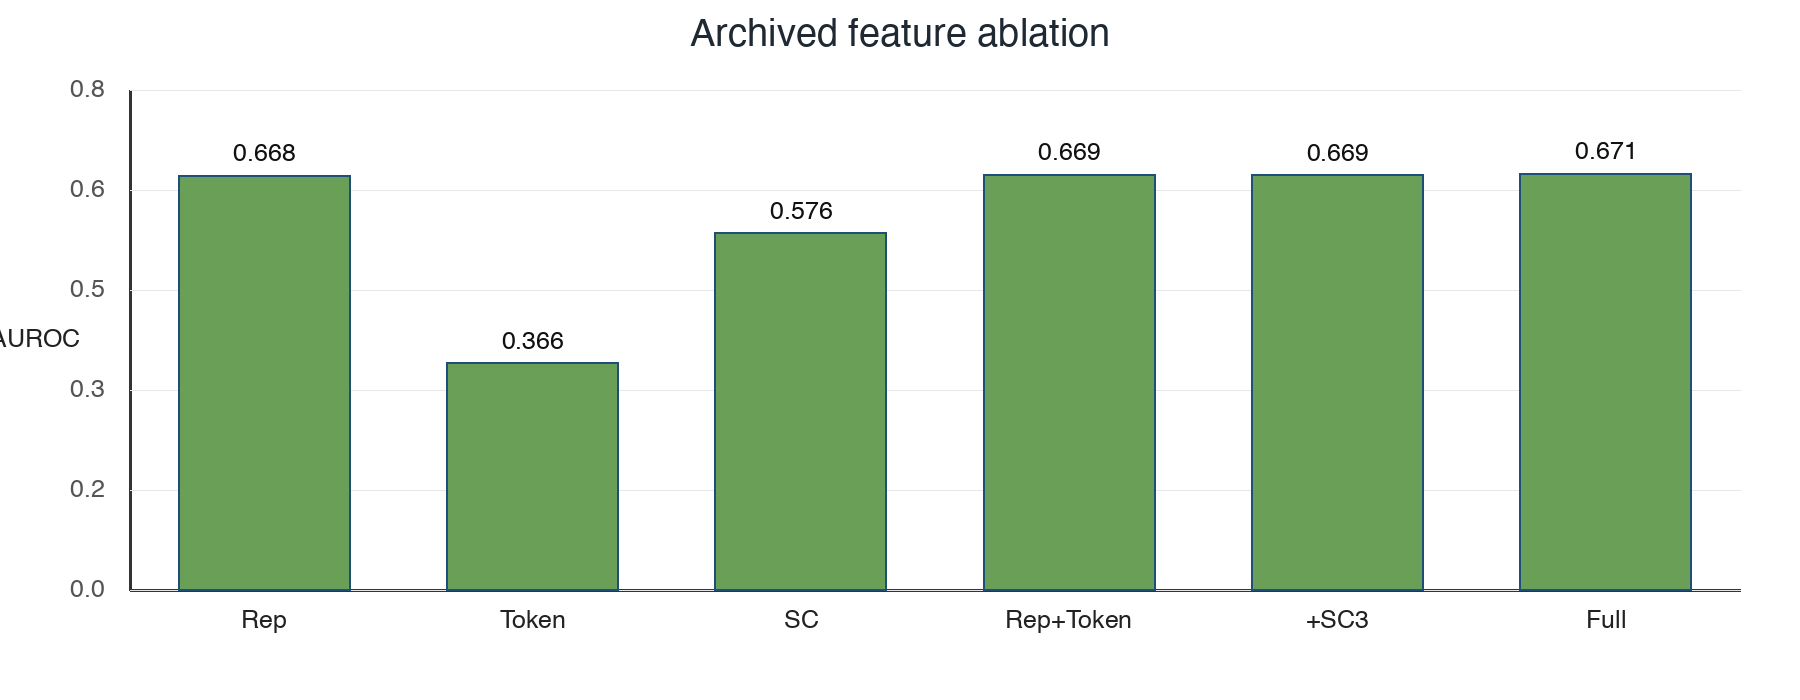
\includegraphics[width=0.80\textwidth]{ablation.png}
\caption{Archived feature-ablation visualization.}
\label{fig:ablation}
\end{figure}

\section{Confusion Analysis and Statistical Evidence}
For the conservative DoLa+ENN+self-consistency setting, the confusion matrix is TP=11, TN=151, FP=6, and FN=43. The policy is therefore highly specific: it accepts only six negative examples, but rejects many positive ones. A paired bootstrap comparison of DoLa+ENN versus DoLa reports an accuracy difference of 0.4692 with a 95\% confidence interval of [0.3762, 0.5556]. McNemar's test reports $p<0.001$. In contrast, the complete architecture differs from DoLa+ENN by -0.0427 accuracy with a 95\% confidence interval of [-0.1043, 0.0099] and $p=0.163$.

\begin{figure}[H]
\centering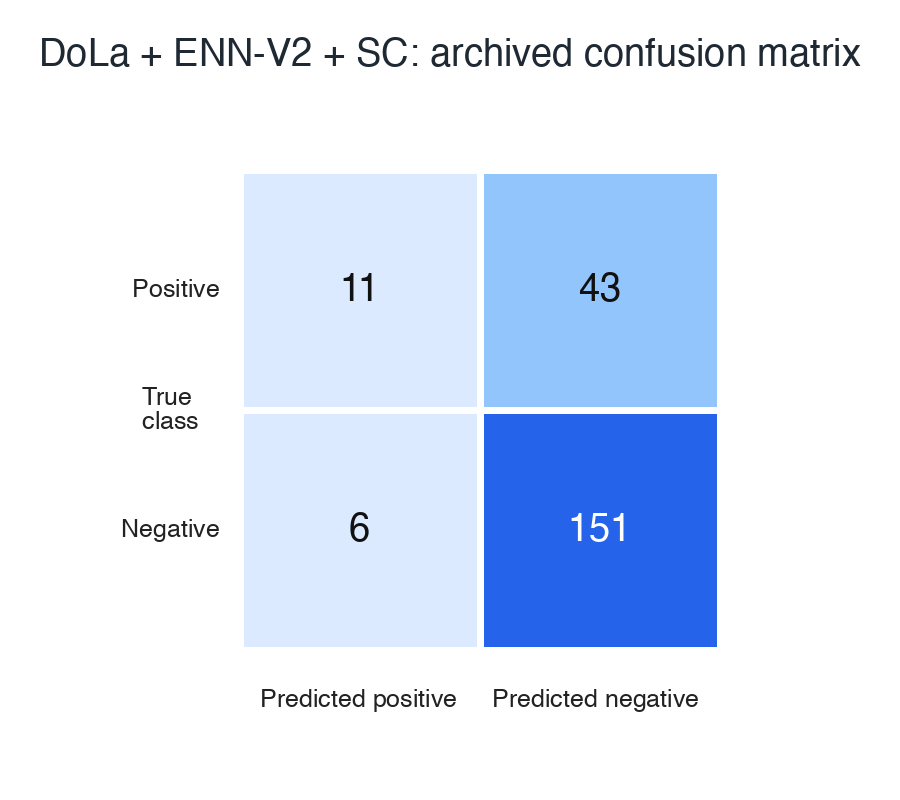
\includegraphics[width=0.68\textwidth]{confusion.png}
\caption{Confusion matrix for the conservative archived reliability decision.}
\label{fig:confusion}
\end{figure}

\section{Limitations}
The current checkout does not contain the trainer source for the upgraded answer-correctness ENN, so archived results cannot be regenerated end to end. The held-out dataset is class-imbalanced, and conservative thresholding improves FAR partly by rejecting many correct answers. The active token-level epinet should not be described as a calibrated answer-correctness model without a supervised validation protocol. Finally, local model behavior, retrieval coverage, and factuality can vary by prompt and domain.

\chapter{CONCLUSION AND FUTURE WORK}
\section{Conclusion}
This Capstone Project presents a hallucination-aware TinyLlama pipeline that combines dynamic layer-contrastive decoding, an epinet with a frozen prior, sampled self-consistency, and a reliability decision layer. The system is designed to make the generation process inspectable through a console that exposes candidate answers and diagnostics. The archived evaluation shows that a conservative DoLa+ENN configuration can sharply reduce false acceptance, but it does so with reduced recall. The evidence supports uncertainty-aware abstention and transparent decision support rather than a broad claim of hallucination elimination.

\section{Future Work}
Future work should recover and archive the upgraded trainer and evaluation code, record dataset revisions and prediction files, and run the complete protocol on larger held-out benchmarks. A dedicated validation set should calibrate thresholds independently from the final test set. Further experiments can compare every-layer versus sparse-layer DoLa selection, calibrated probability models, retrieval-grounded verification, semantic answer equivalence, and risk-coverage curves. Deployment work should also profile latency, memory use, energy cost, and usability on the target hardware.

\appendix
\chapter{USER OPERATING PROCEDURE}
\begin{enumerate}[label=\arabic*.]
\item Launch the local application and verify that the base model and ENN checkpoint status are displayed as loaded.
\item Choose either factuality verification only or context injection plus verification.
\item Set generation controls such as maximum new tokens, temperature, top-$p$, DoLa alpha, self-consistency candidate count, and ENN weight.
\item Enter a question and review the selected final answer together with the verification status.
\item Inspect the pipeline, candidates, claim diagnostics, token uncertainty, and evidence tabs before relying on a response for a high-stakes task.
\item Export the diagnostics when an audit record is required.
\end{enumerate}

\chapter{REPRODUCIBILITY CHECKLIST}
\begin{itemize}
\item Record the exact base-model revision, Python version, library versions, operating system, and accelerator.
\item Preserve C4 source identifiers, data revision, train/validation/test split, random seeds, and all checkpoints.
\item Archive prompt templates, generated candidates, reliability scores, threshold-selection data, and final prediction files.
\item Report both false-accept and false-reject rates, calibration metrics, class distributions, confidence intervals, and paired significance tests.
\item Keep active-source results distinct from any historical archived results whose training code is unavailable.
\end{itemize}

\clearpage
\addcontentsline{toc}{chapter}{References}
\bibliographystyle{plainnat}
\bibliography{references}
\end{document}
